%!TEX root = TNTinderSee.tex 

\chapter[Fazit]{Fazit}

Obwohl unser Untersuchungsgebiet in einem auf Seekarten als \emph{munitionsbelastetet} markiertem Gebiet lag, haben wir trotz aufwändiger Kartierung keine Munition gefunden. Zusätzlich haben uns unsere Wasserproben keinerlei Hinweise auf \emph{sprengstofftypische Verbindungen}, wie man sie in der Nähe von vor-sich-hin rostender Munition erwartet, gezeigt. Betrachtet man die Ergebnisse, wäre die gute Nachricht, dass nicht nur das Gewässer südöstlich von Rügen diesbezüglich unbelastet ist, sondern auch von eventuell nicht aufgespürten Munitionsresten keine Gefahr für das Untersuchungsgebiet zu sein scheint. \\
Andere Untersuchungen kommen allerdings zu anderen Schlüssen, so gilt die Munitionshalde \emph{Kohlberger Heide} in der Kieler Bucht als hochbelastet\cite{kohl} \\
Letztendlich sind unsere Ergebnisse deshalb mit großer Vorsicht zu interpretieren. \\
Eine plausible Erklärung für unsere eigenen Ergebnisse wäre, dass die Reste des o.g. Schutenunglücks zu DDR-Zeiten wieder geborgen wurden und wir deshalb am Ort des Unglücks keine Überreste der Schuten oder der Munition mehr gefunden haben.
Zusätzlich könnte die durch das Flachwasser großzügig vorhandene Biomasse eventuelle Restbelastungen aufgenommen haben. Diese spielt in der Ionenchromatografie wegen der notwendigen Filtrierung der Proben nämlich keine Rolle. \\
Um das zu prüfen, müsste die Biomasse gezielt untersucht werden.\\
Vielleicht waren wir aber auch einfach zu weit weg von der nächsten Munitionshalde.\\
\begin{figure}[htb]
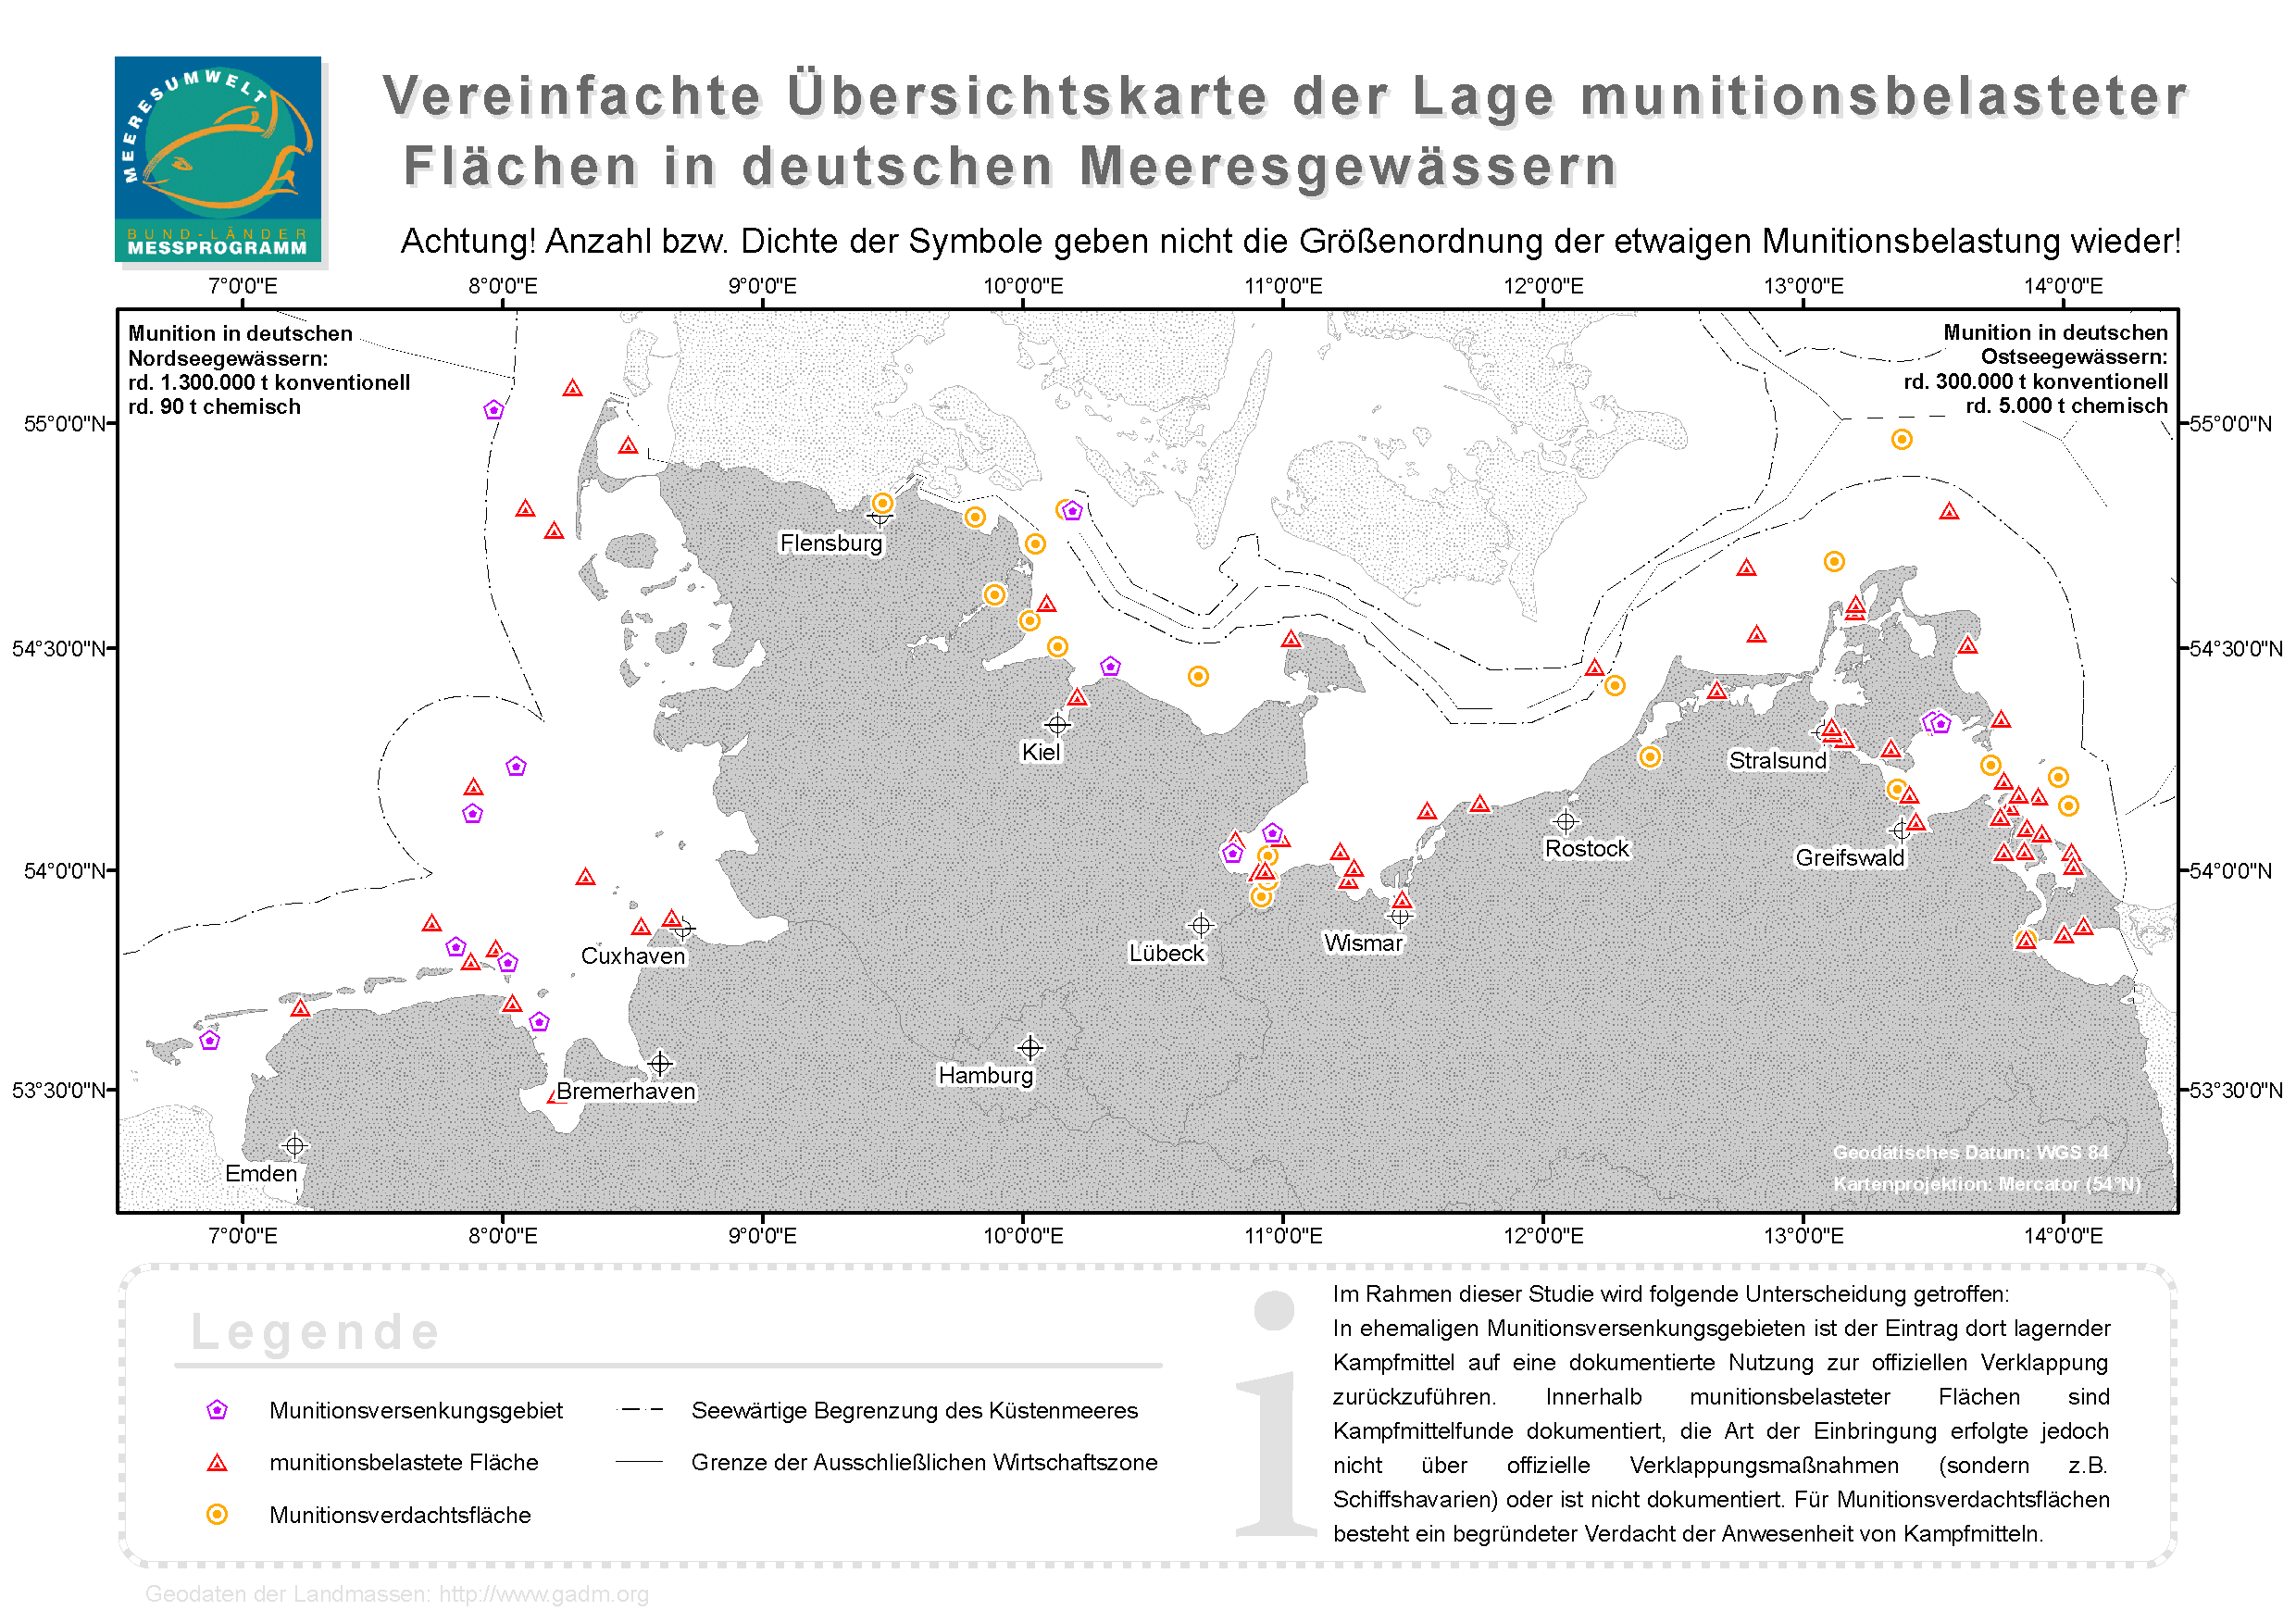
\includegraphics[height=\textheight,%
                   width=\textwidth,%
                   keepaspectratio]{Bilder/karte_muni.PDF}
\caption{Karte der Munitionslagerstätten in Nord- und Ostsee\cite{shmuni}.}
\end{figure}

Trotz unserer Untersuchungsergebnisse bleibt die Gefahr durch Altmunition in der Ostsee weiter bestehen (siehe Abb 4.1.) und es muss dringend ein Konzept zur Bergung und Entsorgung der Munition her, um das Ökosystem Ostsee zu schützen.\\

Diese Forschungsreise war für uns alle eine wunderbare und sicherlich prägende Erfahrung, dafür möchten wir uns bei allen Beteiligten herzlich bedanken.\\

Und falls bei der nächsten Forschungsfrage ein kleiner Tauchroboter inklusive Minicrew benötigt werden sollte: Wir denken, die See schuldet uns noch was. :-)

\begin{figure}[htb]
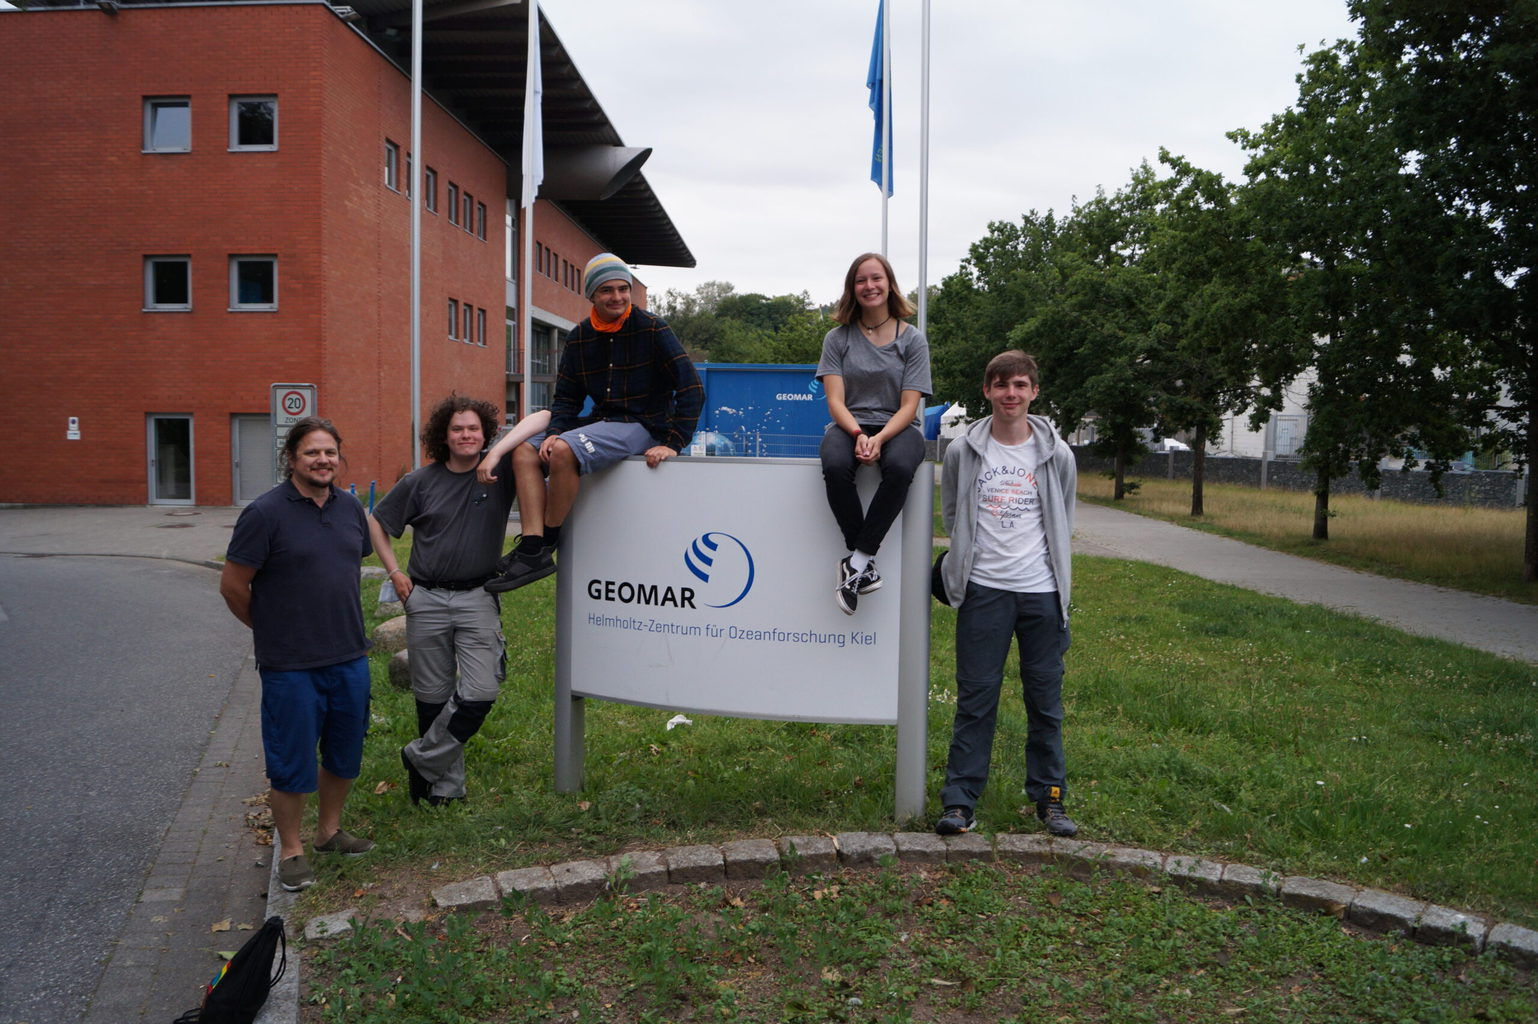
\includegraphics[height=\textheight,%
                   width=\textwidth,%
                   keepaspectratio]{Bilder/ROV/Gruppenfoto}
\caption{Das Forschungsteam (von li.n.re.) Marek Czernohous (Betreuer), Alexander Komyakov, Martin Eitel, Luisa Sauerbrey, Antonio Rehwinkel}
\end{figure}




